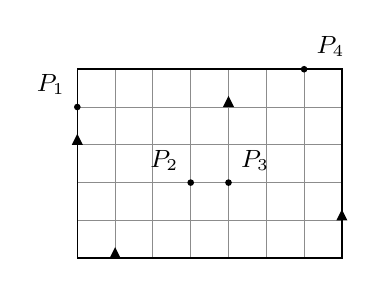
\begin{tikzpicture}[x=0.48cm,y=0.48cm,every node/.style={font=\small}]
  % Seven columns by five rows of unit squares; coordinates are only for redraw.
  \draw[step=1,black!45,line width=0.35pt] (0,0) grid (7,5);
  \draw[line width=0.55pt] (0,0) rectangle (7,5);

  % Marked P-points from the source.
  \fill (0,4) circle (1.2pt);
  \node[above left=1pt] at (0,4) {$P_1$};
  \fill (3,2) circle (1.2pt);
  \node[above left=1pt] at (3,2) {$P_2$};
  \fill (4,2) circle (1.2pt);
  \node[above right=1pt] at (4,2) {$P_3$};
  \fill (6,5) circle (1.2pt);
  \node[above right=1pt] at (6,5) {$P_4$};

  % The four solid triangles occupy the source lattice vertices.
  \fill (1,0) ++(-2pt,0) -- ++(2pt,4pt) -- ++(2pt,-4pt) -- cycle;
  \fill (0,3) ++(-2pt,0) -- ++(2pt,4pt) -- ++(2pt,-4pt) -- cycle;
  \fill (4,4) ++(-2pt,0) -- ++(2pt,4pt) -- ++(2pt,-4pt) -- cycle;
  \fill (7,1) ++(-2pt,0) -- ++(2pt,4pt) -- ++(2pt,-4pt) -- cycle;
\end{tikzpicture}
